\documentclass[11pt]{report}
%%% Packages
\usepackage{amsmath,amsthm,amssymb,amsfonts}
\usepackage{graphicx}
\usepackage{xspace}
\usepackage{xcolor}
\usepackage[
	pdftitle=Project,
	colorlinks=false,
	final,
	linkcolor=blue,
	citecolor=magenta,
	urlcolor=blue,
]{hyperref}
\usepackage[obeyDraft, textsize=footnotesize, colorinlistoftodos]{todonotes}
\usepackage{verbatim}
\usepackage{enumitem}
\usepackage[toc]{appendix}
\usepackage{array}
\usepackage{cancel}
\usepackage{framed}

\setlist[enumerate,1]{label=(\arabic*)} % to make basic enumerate with 1) instead of 1.


\renewcommand{\thesection}{\arabic{section}}
\renewcommand{\thesubsection}{\thesection.\arabic{subsection}}
\renewcommand{\thesubsubsection}{\thesubsection.\arabic{subsubsection}}


\hbadness=10000

\usepackage{multicol}
\usepackage[
	paper=a4paper, % Change to letterpaper for US letter
	bottom=3cm, % Bottom margin
]{geometry} %% geomatry dash??

\usepackage{soul} %% like Aretha Franklin??
\usepackage{multicol}
\usepackage[skip=5pt plus1pt, indent=0pt]{parskip}
\usepackage{realhats}

\usepackage{multirow}
\usepackage{tikz-cd} % sonic cd???
\usetikzlibrary{graphs, 3d} % i put this here btw

%\usepackage[square,numbers]{natbib}%, sorting=nyt]
\usepackage[style=numeric, backend=biber, sorting=nyt]{biblatex}
\addbibresource{refs.bib}

\usepackage{float,caption}

%%%%% fancy hdr and sections
\usepackage{titlesec}
\titleformat{\chapter}
{\normalfont\huge\bfseries}{\chaptertitlename\ \thechapter.}{1em}{}

\usepackage{fancyhdr}
\pagestyle{fancy}
\fancyhf{}
\setlength{\headheight}{14pt}

\makeatletter
\renewcommand{\sectionmark}[1]{\markright{\thesection~~~#1}}
\renewcommand{\chaptermark}[1]{\markboth{\if@mainmatter \fi#1}{}}
\makeatother

\makeatletter
\newcommand{\chapterauthor}[1]{%
	{\parindent0pt\vspace*{-25pt}%
			\linespread{1.1}\Large\centering#1%
			\par\nobreak\vspace*{35pt}}
	\@afterheading%
}
\makeatother


% part title in each part
\fancyhead[L]{\nouppercase{\leftmark}}
\fancyhead[R]{Invariant Theory}
\cfoot{\thepage}

\newcommand{\Sn}[1][n]{\mathcal{S}_{#1}\xspace}
\newcommand{\An}[1][n]{\mathcal{A}_{#1}\xspace}
\newcommand{\set}[1]{\ensuremath{\left\lbrace #1 \right\rbrace}\xspace}

\newcommand\restr[2]{{% we make the whole thing an ordinary symbol
\left.\kern-\nulldelimiterspace % automatically resize the bar with \right
#1 % the function
\littletaller % pretend it's a little taller at normal size
\right|_{#2} % this is the delimiter
}}
\newcommand{\littletaller}{\mathchoice{\vphantom{\big|}}{}{}{}}


%%% ===== Styling for theorems
\theoremstyle{plain} % the style for theorem, propositions and lemmas
% Counter used to make it continuous numbering with subsubsection value appended
\newtheorem{thm}{Theorem}[section] % name shortcut for Theorem & counter check
\newtheorem{theorem}[thm]{Theorem}
\newtheorem{prop}[thm]{Proposition}
\newtheorem{proposition}[thm]{Proposition}
\newtheorem{lem}[thm]{Lemma}
\newtheorem{lemma}[thm]{Lemma}
\newtheorem{cor}[thm]{Corollary}
\newtheorem{corollary}[thm]{Corollary}
\newtheorem{conj}[thm]{Conjecture}
\newtheorem{claim}{Claim}
\newcounter{scount}[subsection] % counter to only go down to subsection but make it different
\renewcommand{\thescount}{\arabic{subsection}.\arabic{scount}}
\newtheorem{scholie}[scount]{Scholie}
\theoremstyle{definition} % the style for definitions
\newtheorem{defn}[thm]{Definition} % shortname
\newtheorem{definition}[thm]{Definition} % shortname
\newtheorem*{defns}{Definitions} % plural shortname
\newtheorem{ex}[thm]{Example}
\newtheorem{example}[thm]{Example}
\theoremstyle{remark} % the style for remarks and examples
\newtheorem{rem}[thm]{/emark} % shortname
\newtheorem{remark}[thm]{Remark} % longname
\newtheorem*{rem*}{Remark} % starred version
\newtheorem*{note}{Note}
\newtheorem*{rems}{Remarks} % plural
\newtheorem{notation}[thm]{Notation}
\newtheorem*{notation*}{Notation}
\newtheorem{question}[thm]{Question}
\counterwithin{equation}{section}
\counterwithin{figure}{section}

%%% Shorthands
\newcommand{\N}{\ensuremath{\mathbb{N}}}
\newcommand{\Z}{\ensuremath{\mathbb{Z}}}
\newcommand{\Q}{\ensuremath{\mathbb{Q}}}
\newcommand{\R}{\ensuremath{\mathbb{R}}}
\newcommand{\C}{\ensuremath{\mathbb{C}}}
\newcommand{\F}{\ensuremath{\mathbb{F}}}
\newcommand{\Card}[1]{\lvert #1 \rvert}
\newcommand{\priv}{\setminus}
\newcommand{\ob}[1]{\overline{#1}}
\newcommand{\ssi}{\Leftrightarrow}
\newcommand{\g}{\mathbf{g}}

%% Math Operators

\DeclareMathOperator{\GL}{GL}
\DeclareMathOperator{\Dim}{Dim}
\DeclareMathOperator{\Rank}{Rank}
\DeclareMathOperator{\Ham}{Ham}
\DeclareMathOperator{\Fix}{Fix}
\DeclareMathOperator{\Jac}{Jac}


%%% Todo notes
% Colouring
\def\mathcolor#1#{\@mathcolor{#1}}
\def\@mathcolor#1#2#3{%
	\protect\leavevmode
	\begingroup\color#1{#2}#3\endgroup
}
\newcommand{\blue}[1]{\mathcolor{blue}{#1}}
\newcommand{\rose}[1]{\mathcolor{magenta}{#1}}

% Todo items
\definecolor{cadetblue}{rgb}{0.37, 0.62, 0.63} % ocean blue
\definecolor{celadon}{rgb}{0.67, 0.88, 0.69} % light green
\definecolor{arylide}{rgb}{0.91, 0.84, 0.42} % mustardy yellow
\newcommand{\checkref}[2][]{\todo[color=cadetblue, #1]{#2}}
\newcommand{\suggestion}[2][]{\todo[color=celadon, inline, #1]{#2}}
\newcommand{\idea}[2][]{\todo[color=magenta!70!black, #1]{#2}}
\newcommand{\error}[2][]{\todo[color=red!70, #1]{#2}}


%% If you want to add packages add them under THIS LINE
%% They will get edited later


%\setcounter{section}{0}}

\title{\Huge\textbf{Formal Languages and Automata Theory}}
\author{\large Akash Gopinath}
\date{\today}


\begin{document}

{
\let\newpage\relax
\maketitle
\begin{center}
	\vfill
	\Large
	MMath Independent Project \\
	Supervised by Prof. Victoria Gould

	\vspace{0.4cm}
	
\includegraphics[width=0.5\textwidth]{university.png}

	\textbf{
		Department of Mathematics \\
		University of York \\
		2025 - 2026	}
\end{center}
}
\titlepage

\pagestyle{fancy}

%\begin{abstract}
%\end{abstract}

\tableofcontents
\newpage

%\chapter{Introduction}

%\input{Sections/introduction}
%\newpage

\chapter{What is my project}
My topic is on the study of formal languages and automata theory. This topic is an intersection of mathematics and theoretical computer science. It explores the relationship between
algebraic structures and computational models, providing a rigorous framework for understanding the capabilities and limitations of different types of automata and the languages they recognize.

A DFA, or Deterministic Finite Automata, is a theoretical model of computation that consists of a finite set of states, an input alphabet, a transition function, a start state, and a set of accept states. A DFA can also be viewed as a generator of algebraic information.
A regular language $L$ has associated with it a monoid $M(L)$ called the syntactic monoid of L.
Monoids help us determine the class of regular recognizable languages.

My first objective is to understand the algebraic structure of $M(L)$ and then use this to study varieties and pseudovarieties of monoids.
A variety of algebras is a class of algebras closed under the formation of homomorphic images, subalgebras, and arbitrary direct products. When restricted to finite algebras, these are called pseudovarieties.

The next objective is to explore Eilenberg's correspondence, which establishes a bijective relationship between varieties of regular languages and pseudovarieties of finite monoids.
This correspondence allows us to translate problems in language theory into problems in algebra and vice versa, providing powerful tools for analysis. Under this correspondence, a regula language $L$
belongs to a variety of languages $\mathcal{V}$ if and only if its syntactic monoid $M(L)$ belongs to the corresponding pseudovariety of monoids $\mathcal{W}$.

This connection is useful in classifying regular languages based on the algebraic properties of their syntactic monoids.

An important result in this area is Rietterman's theorem. This theorem states that a class of monoids is a pseudovariety if and only if it can be defined by a set of profinite identities. This is useful in the membership problem for pseudovarieties of finite monoids 
as it provides a way to characterize pseudovarieties using identities, which can be easier to work with than directly dealing with the monoids themselves.

Finally I would like to look into the membership problem for pseudovarieties of finite monoids. Which is the problem of determining whether a given finite monoid belongs to a specified pseudovariety.
This problem has significant implications in automata theory and formal language theory. I would also like to look into algorithms used in the membership problem for certain pseudovarities.

\begin{framed}
    The aim of this project is to explore pseudovarieties of finite monoids and their applications in formal languages and automata theory.
\end{framed}

\newpage



\chapter{How I will achieve this}
I have already finished reading through the relevant lecture notes provided by my supervisor. These notes cover the key concepts and techniques in formal languages and automata theory.

The next step is to delve deeper into the topic of varieties of formal languages. I am currently studying a book titled ``Varieties of Formal Languages" by Jean-Éric Pin. This book provides a comprehensive overview of the theory of varieties and their applications in formal languages.
This text will be the main reference for understanding how regular languages can be classified using algebraic structures.

In addition to this, I plan to consult the following textbooks/research methods:
\begin{itemize}
    \item Samuel Eilenberg's ``Automata, Languages, and Machines" which provides foundational knowledge on automata theory and formal languages.
    \item John M. Howie's ``Automata and Languages" which is a gentle introduction to the subject.
    \item I will also look into research papers into the membership problem for pseudovarieties of finite monoids to understand the current state of research in this area.
\end{itemize}

Using literature, I will do 2 things:

\begin{enumerate}
    \item {\bf Theoretical study:} I will study the structure of the syntactic monoid of regular languages and understand how varieties and pseudovarieties are defined and classified. I will explore Eilenberg's correspondence in detail and understand how it can be used to classify regular languages based on the properties of their syntactic monoids.
    \item {\bf Computational study:} I will use computational tools such as GAP (Groups, Algorithms and Programming) to experiment and compute syntactic monoids of regular languages of small DFAs. I will try to implement algorithms to test membership in certain pseudovarieties of finite monoids and analyze their efficiency and effectiveness. Through this I want to shed light on the membership problem and see if it will yield new examples/insights.
\end{enumerate}

{\bf Where things might go wrong:}
\begin{itemize}
    \item Might be a bit too ambitious in terms of the scope of the project. The theoretical study might take longer than expected, leaving less time for the computational study.
    \item The computational study may face challenges such as the limitations of the GAP system or the complexity of the algorithms to implemented. This could result in incomplete or inaccurate findings.
\end{itemize}
\newpage

\chapter{Motivations and issues I hope to address}
%\chapter{What I hope to do in my project}
The reason I am doing this topic is because I find it interesting how algebraic structures such as monoids can be used to classify and understand formal languages and automata. 
Eilenberg's correspondence is a powerful tool that connects these two areas, allowing for a deeper understanding of the properties of regular languages through the lens of algebra.
For example star free languages correspond to aperiodic monoids.

This topic has both theoretical and computational aspects which I can explore which makes it appealing to me. Also after taking
a course on semigroup theory last year, I developed a fascination in the subject and would like to explore its applications in automata theory.

\section*{Issues I hope to address}
The are several issues I hope to address in this project:
\begin{itemize}
    \item {\bf Scope:} The scope of the project is quite large. It might take a lot to build up to Eilenberg's correspondence and the membership problem may be too ambitious to tackle in the time frame. 
    Nevertheless, even with Eilenberg's correspondence alone, I can gain a lot of insight into the classification of regular languages and could do a broad survey of membership without trying to implement algorithms.
    \item {\bf Computational challenges:} Implementing algorithms to test membership in pseudovarities may be too complex in the time frame I am given. But I still hope to tryt and compute syntactic monoids of small DFAs using GAP since that is a finite simple process.
    \item {\bf Timeframe I have set for the literature:} In the gantt chart below, I have outlined when I hope to what task. But it is based on my current understanding of the topic. As I read more literature, I may find that some topics take longer to understand than I initially thought.
    It may take longer also due to lectures, exams and other commitments. I will try to manage my time effectively to ensure I can cover the necessary material within the timeframe. 
 \end{itemize}

 But overall, I can definitely get to Eilenberg's correspondence and understand how varieties of regular languages and pseudovarieties of finite monoids are connected. And then just do a broad survey of membership of known pseudovarieties.

 In testing membership, Reiterman's theorem is useful. But I will be omitting the details of profinite identities in this project since the topological arguments are not in the scope of this project.
\newpage

\chapter{Timeline of the project}
Here is a Gantt chart showing the timeline for my MMath independent project:


\begin{figure}[h] % 'h' means place it here
    \centering
    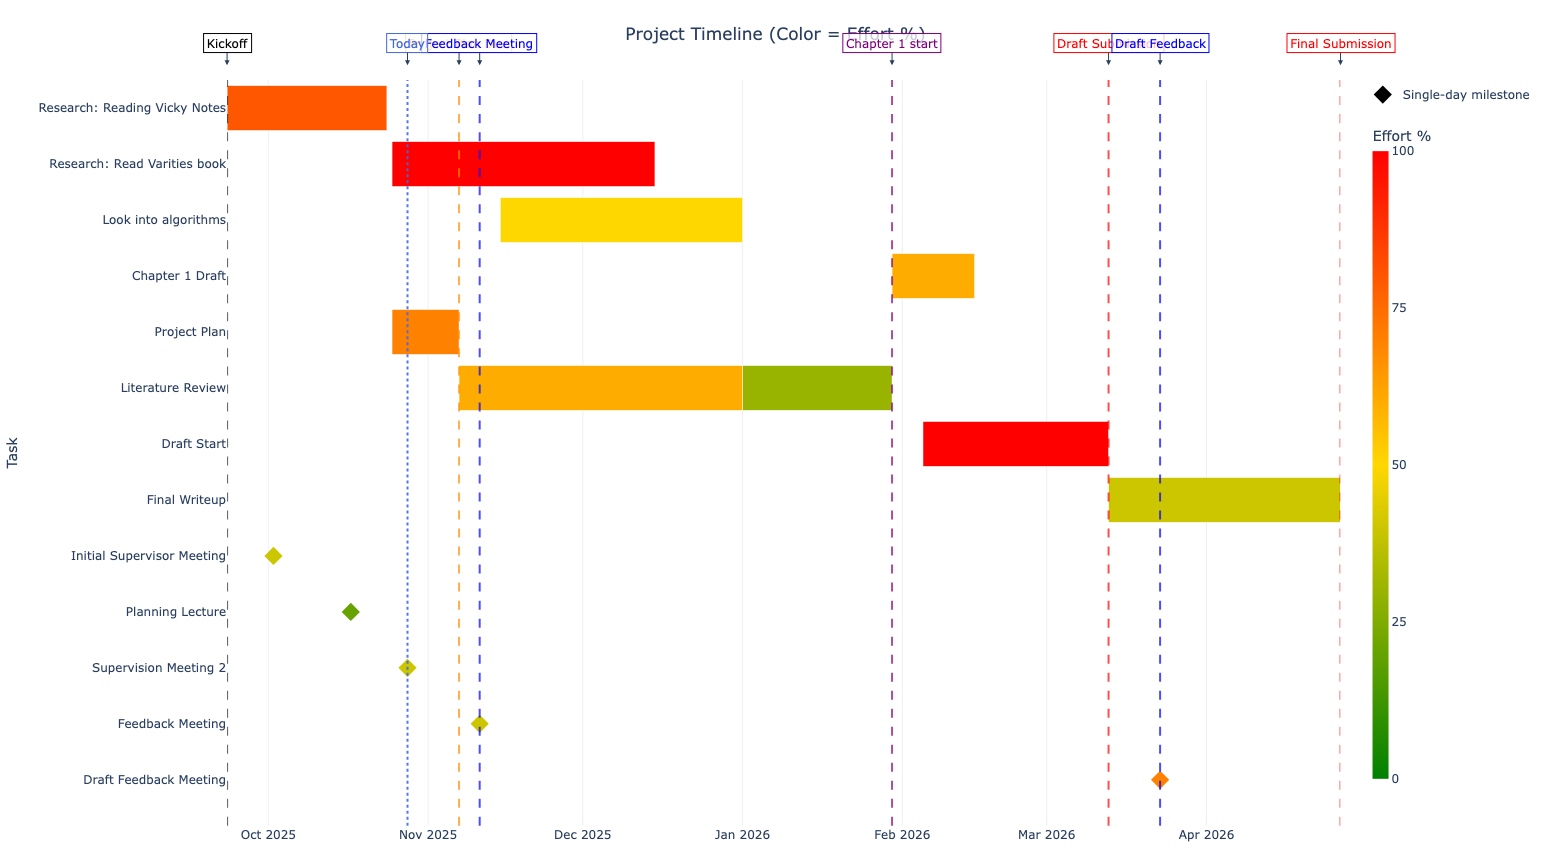
\includegraphics[width=1.2\textwidth]{newplot(3)} % image file name without extension
    \caption{Gantt chart showing the timeline for the MMath independent project.}
    \label{fig:gantt_chart}
\end{figure}

% Make a box with a URL link to interactive Gantt chart
\begin{center}
	\fbox{\parbox{0.9\textwidth}{
		For an interactive version of this Gantt chart, please visit: \\
		\centering
		\url{https://www-users.york.ac.uk/~ag1884/}
	}}
\end{center}

\section*{Written Commentary of plan}
The Gantt chart in Figure~\ref{fig:gantt_chart} outlines the timeline for my MMath independent project. The project is structured into several key phases, each with specific tasks and milestones.

\begin{itemize}
	\item \textbf{Initial Research (Weeks 1-5):}  During this part, I focused on reading the lecure notes of my supervisor Prof Victoria Gould and relevant material from book "Automata and Languages" by John M. Howie. This helped me understand the basics of DFA's and syntactic monoids
	\item \textbf{Project Plan (Weeks 5-6)}: I started working on my project plan. This also relied on me consulting additonal literaturein tandem.
	\item \textbf{Study on Varieties (Weeks 6-12):} This phase involves a deep dive into the theoretical and computational aspects of pseudovarieties of finite monoids and their applications in formal languages and automata theory. I will study Eilenberg's correspondence and related concepts. Most of this material is covered in the book "Varieties of Formal Languages" by Jean-Éric Pin and his lecture notes available online.
	\begin{itemize}
		\item October 25-December 15: Read through relevant chapters of Jean-Éric Pin's book and understand the theoretical concepts.
		\item November 15-January 1: Look into algorithms used to generate syntactic monoids of regular languages and test membership in pseudovarieties.
	\end{itemize}
	
\end{itemize}
\newpage



%\chapter{Conclusion}
\input{Sections/footer}


\newpage
\setcounter{chapter}{9}
%\renewcommand{\chaptertitle}{Bibliography}
% \bibliographystyle{plainnat}
% \bibliographystyle{unsrtnat}
% \bibliography{refs}
\printbibliography

\appendix
\input{Sections/appendix.tex}

\end{document}

